\subsection{题目描述}
\noindent
Solve the time-dependent Schrödinger equation using both the Crank–Nicolson scheme and a stable explicit scheme. Consider the one-dimensional case and test it by applying it to the problem of a square well with a Gaussian initial state coming in from the left.

\noindent
Hint: The Gaussian initial state could be expressed as:
\[
    \Psi(x, 0) = \sqrt{\frac{1}{\pi}} \exp\left[ i k_0 x - \frac{(x - \xi_0)^2}{2} \right].
\]


\subsection{程序描述}
本程序通过\texttt{Parameters}类管理参数,包括网格参数(时空坐标剖分)、势阱参数(宽度、深度与中心位置)以及初始波包参数(宽度、位置与动量)。定义了一个\texttt{SchrodingerSolver}求解器基类,包含了Crank–Nicolson解法与显式解法的接口,以及一些共用的方法,如检查输入参数是否满足Von Neumann稳定性条件。两个求解器\texttt{CrankNicolsonSolver}与\texttt{ExplicitSolver}继承自基类,分别实现了Crank–Nicolson解法与显式解法。本题求解的一维含时薛定谔方程
\[
    i\hbar \frac{\partial \psi(x,t)}{\partial t} = -\frac{\hbar^2}{2m} \frac{\partial^2 \psi(x,t)}{\partial x^2} + V(x) \psi(x,t)
\]在原子单位制$\hbar = m =1$下化简为
\[
    i \frac{\partial \psi}{\partial t} = -\frac{1}{2} \frac{\partial^2 \psi}{\partial x^2} + V(x) \psi
\]
离散化时记 $\psi_j^n$ 为在位置 $x_j = j \Delta x $和时间 $t^n = n \Delta t $处的波函数值。
\subsubsection{Crank-Nicolson算法}
类比二阶偏微分方程中的Gauss-Seidel迭代,隐式的Crank-Nicolson 算法对时间导数采用前向差分,对中心差分的空间导数和势能项取时间切片 \(n\) 和 \(n+1\) 的平均,即:
\[
    i \frac{\psi_j^{n+1} - \psi_j^n}{\Delta t} = -\frac{1}{4} \left( \frac{\psi_{j+1}^{n+1} - 2\psi_j^{n+1} + \psi_{j-1}^{n+1}}{(\Delta x)^2} + \frac{\psi_{j+1}^n - 2\psi_j^n + \psi_{j-1}^n}{(\Delta x)^2} \right) + \frac{1}{2} V_j \left( \psi_j^{n+1} + \psi_j^n \right)
\]
可以整理为半步演化形式
\[
    \left( 1 + i \frac{\Delta t}{2} \hat{H} \right) \psi^{n+1} = \left( 1 - i \frac{\Delta t}{2} \hat{H} \right) \psi^n
\]
其中哈密顿算符在每个时间切片上离散化为
\[
    \hat{H} \psi_j = -\frac{1}{2 (\Delta x)^2} \left( \psi_{j+1} - 2\psi_j + \psi_{j-1} \right) + V_j \psi_j
\]
实际代码实现中,构造了两个三对角矩阵,化方程为$\mathbf{A} \psi^{n+1} = \mathbf{B} \psi^n$,满足$\mathbf{A} = \mathbf{I} + i \frac{\Delta t}{2} \mathbf{H}\text{与}\mathbf{B} = \mathbf{I} - i \frac{\Delta t}{2} \mathbf{H}$,即
\[
    \mathbf{A}, \mathbf{B} =
    \begin{pmatrix}
        1 + 2\alpha \pm \frac{i \Delta t}{2} V_1 & \mp \alpha                               & 0                                        & \cdots     & 0                                            \\
        \mp \alpha                               & 1 + 2\alpha \pm \frac{i \Delta t}{2} V_2 & \mp \alpha                               & \ddots     & \vdots                                       \\
        0                                        & \mp \alpha                               & 1 + 2\alpha \pm \frac{i \Delta t}{2} V_3 & \ddots     & 0                                            \\
        \vdots                                   & \ddots                                   & \ddots                                   & \ddots     & \mp \alpha                                   \\
        0                                        & \cdots                                   & 0                                        & \mp \alpha & 1 + 2\alpha \pm \frac{i \Delta t}{2} V_{N_x} \\
    \end{pmatrix}
\]
其中$
    \alpha = \frac{i \Delta t}{4 (\Delta x)^2}
$,模长需满足Von Neumann稳定性条件。

在演化步骤中,三对角矩阵均使用 \texttt{CSC} 稀疏格式存储,并使用 \texttt{scipy.sparse.linalg.spsolve} 进行求解,以提高计算效率和节省内存。
\subsubsection{显式算法}
显式算法对时间导数与空间导数采用中心差分,但不对相邻切片的势能或者空间导数进行平均
\[
    i \frac{\psi_j^{n+1} - \psi_j^{n-1}}{2\Delta t} = -\frac{1}{2} \frac{\psi_{j+1}^n - 2\psi_j^n + \psi_{j-1}^n}{(\Delta x)^2} + V_j \psi_j^n
\]
故可以直接进行显式更新
\[
    \psi_j^{n+1} = \psi_j^{n-1} + \frac{i \Delta t}{\Delta x^2} \left( \psi_{j+1}^n + \psi_{j-1}^n - 2\psi_j^n \right) - 2i \Delta t V_j \psi_j^n
\]
化为矩阵形式即为
\[
    \psi^{n+1} = \psi^{n-1} + \frac{i \Delta t}{(\Delta x)^2} \mathbf{L} \psi^n - 2i \Delta t \mathbf{V} \psi^n
\]
其中$\mathbf{V}$即离散的势能项,动能项为拉普拉斯算符
\[
    \mathbf{L} =
    \begin{pmatrix}
        -2     & 1      & 0      & \cdots & 1      \\
        1      & -2     & 1      & \cdots & 0      \\
        0      & 1      & -2     & \cdots & 0      \\
        \vdots & \ddots & \ddots & \ddots & \vdots \\
        1      & 0      & 0      & 1      & -2
    \end{pmatrix}
\]
实际代码实现中没有显式定义$\mathbf{L}$,而是在每一步中借助\texttt{np.roll}函数(将数组在周期边界条件下顺次移动),直接计算了$\mathbf{L} \psi^n$。在第一步中因为没有$\psi^{n-1}$,故使用Crank-Nicolson算法进行第一步演化,之后都使用显式算法进行演化。
\subsection{伪代码}
Powered by \href{https://chatgpt.com/g/g-xJJAA2awf-latex-pseudocode-generator}{\LaTeX \ pseudocode generator}

\begin{algorithm}[H]
    \SetAlgoLined
    \SetKwFunction{spsolve}{spsolve}
    \KwIn{$\psi$ (initial wave function), $\Delta t$, $\Delta x$, $V$ (potential), $N_x$ (spatial resolution), $N_t$ (time steps)}
    \KwOut{$\psi_{\text{history}}$ (wave function at all time steps)}
    \BlankLine

    $\alpha \leftarrow i \Delta t / (4 \Delta x^2)$ \tcp*[r]{Precompute coefficient}
    $\mathbf{A} \leftarrow \text{ConstructMatrix}([- \alpha, 1 + 2\alpha + i \Delta t V / 2, - \alpha], [-1, 0, 1], N_x)$ \tcp*[r]{Left-hand matrix}
    $\mathbf{B} \leftarrow \text{ConstructMatrix}([\alpha, 1 - 2\alpha - i \Delta t V / 2, \alpha], [-1, 0, 1], N_x)$ \tcp*[r]{Right-hand matrix}

    % $\psi_{\text{history}} \leftarrow [\psi]$ \tcp*[r]{Record initial wave function}

    \For{$t \leftarrow 1$ \KwTo $N_t - 1$}{
        $\psi \leftarrow \spsolve(\mathbf{A}, \mathbf{B} \cdot \psi)$ \tcp*[r]{Solve $\mathbf{A} \psi^{(n+1)} = \mathbf{B} \psi^{(n)}$}
        Append $\psi$ to $\psi_{\text{history}}$ \tcp*[r]{Record updated wave function}
    }

    \Return $\psi_{\text{history}}$
    \caption{Crank-Nicolson Method for Time Evolution (Optimized)}
\end{algorithm}

\begin{algorithm}[H]
    \SetAlgoLined
    \SetKwFunction{spsolve}{spsolve}
    \SetKwFunction{roll}{np.roll}
    \KwIn{$\psi$ (initial wave function), $\Delta t$, $\Delta x$, $V$ (potential), $N_x$ (spatial resolution), $N_t$ (time steps)}
    \KwOut{$\psi_{\text{history}}$ (wave function at all time steps)}
    \BlankLine

    $\alpha \leftarrow i \Delta t / \Delta x^2, \psi_{\text{prev}} \leftarrow \psi, \psi_{\text{history}} \leftarrow [\psi]$ \tcp*[r]{Initialize constants and history}

    \SetKwFunction{CrankNicolsonStep}{CrankNicolsonStep}
    $\psi \leftarrow \CrankNicolsonStep(\psi, \Delta t, \Delta x, V)$ \tcp*[r]{Perform first step using CN method}
    Append $\psi$ to $\psi_{\text{history}}$ \tcp*[r]{Subsequent steps using explicit method}
    \For{$t \leftarrow 2$ \KwTo $N_t - 1$}{
        $\psi_{\text{current}} \leftarrow \psi, \psi_{\text{jp1}} \leftarrow \roll(\psi_{\text{current}}, 1), \psi_{\text{jm1}} \leftarrow \roll(\psi_{\text{current}}, -1)$ \tcp*[r]{Compute shifts}
        $\mathbf{L} \psi^n \leftarrow \psi_{\text{jp1}} + \psi_{\text{jm1}} - 2 \psi_{\text{current}}$ \tcp*[r]{Laplacian action}
        $\psi \leftarrow \psi_{\text{prev}} + \alpha \cdot (\mathbf{L} \psi^n) - 2i \Delta t V \cdot \psi_{\text{current}}$ \tcp*[r]{Update $\psi^{(n+1)}$}
        $\psi_{\text{prev}} \leftarrow \psi_{\text{current}}$ \tcp*[r]{Update $\psi^{(n-1)}$ for next step}
        Append $\psi$ to $\psi_{\text{history}}$ \tcp*[r]{Record updated wave function}
    }

    \Return $\psi_{\text{history}}$
    \caption{Explicit Time Evolution with Crank-Nicolson First Step (Optimized)}
\end{algorithm}

\subsection{结果示例}
\begin{figure}[H]
    \centering
    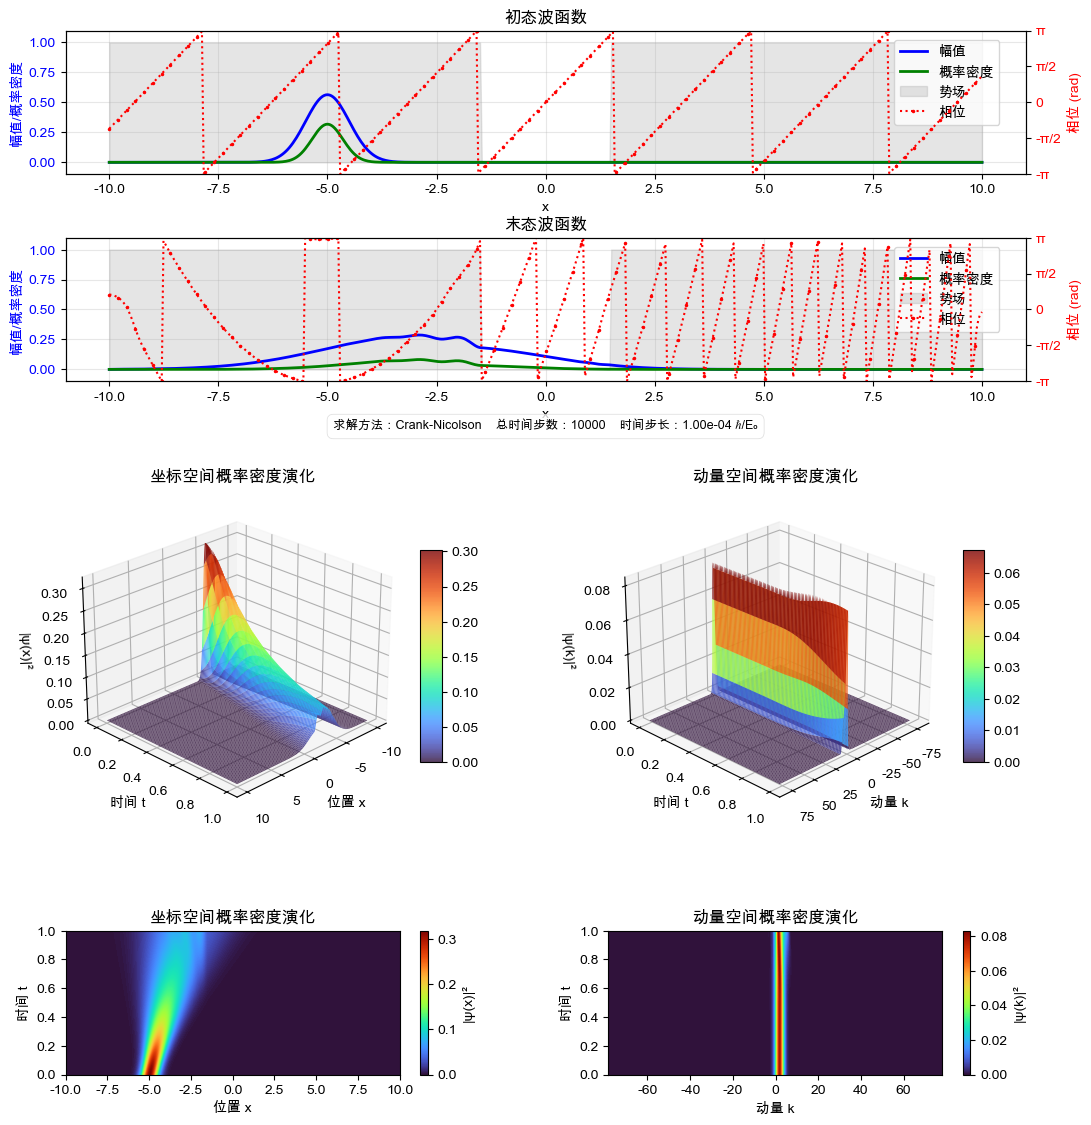
\includegraphics[width=1.0\textwidth]{Problem_2/figs/cn_result.png}
    \caption{Crank–Nicolson解法结果}
\end{figure}

\begin{figure}[H]
    \centering
    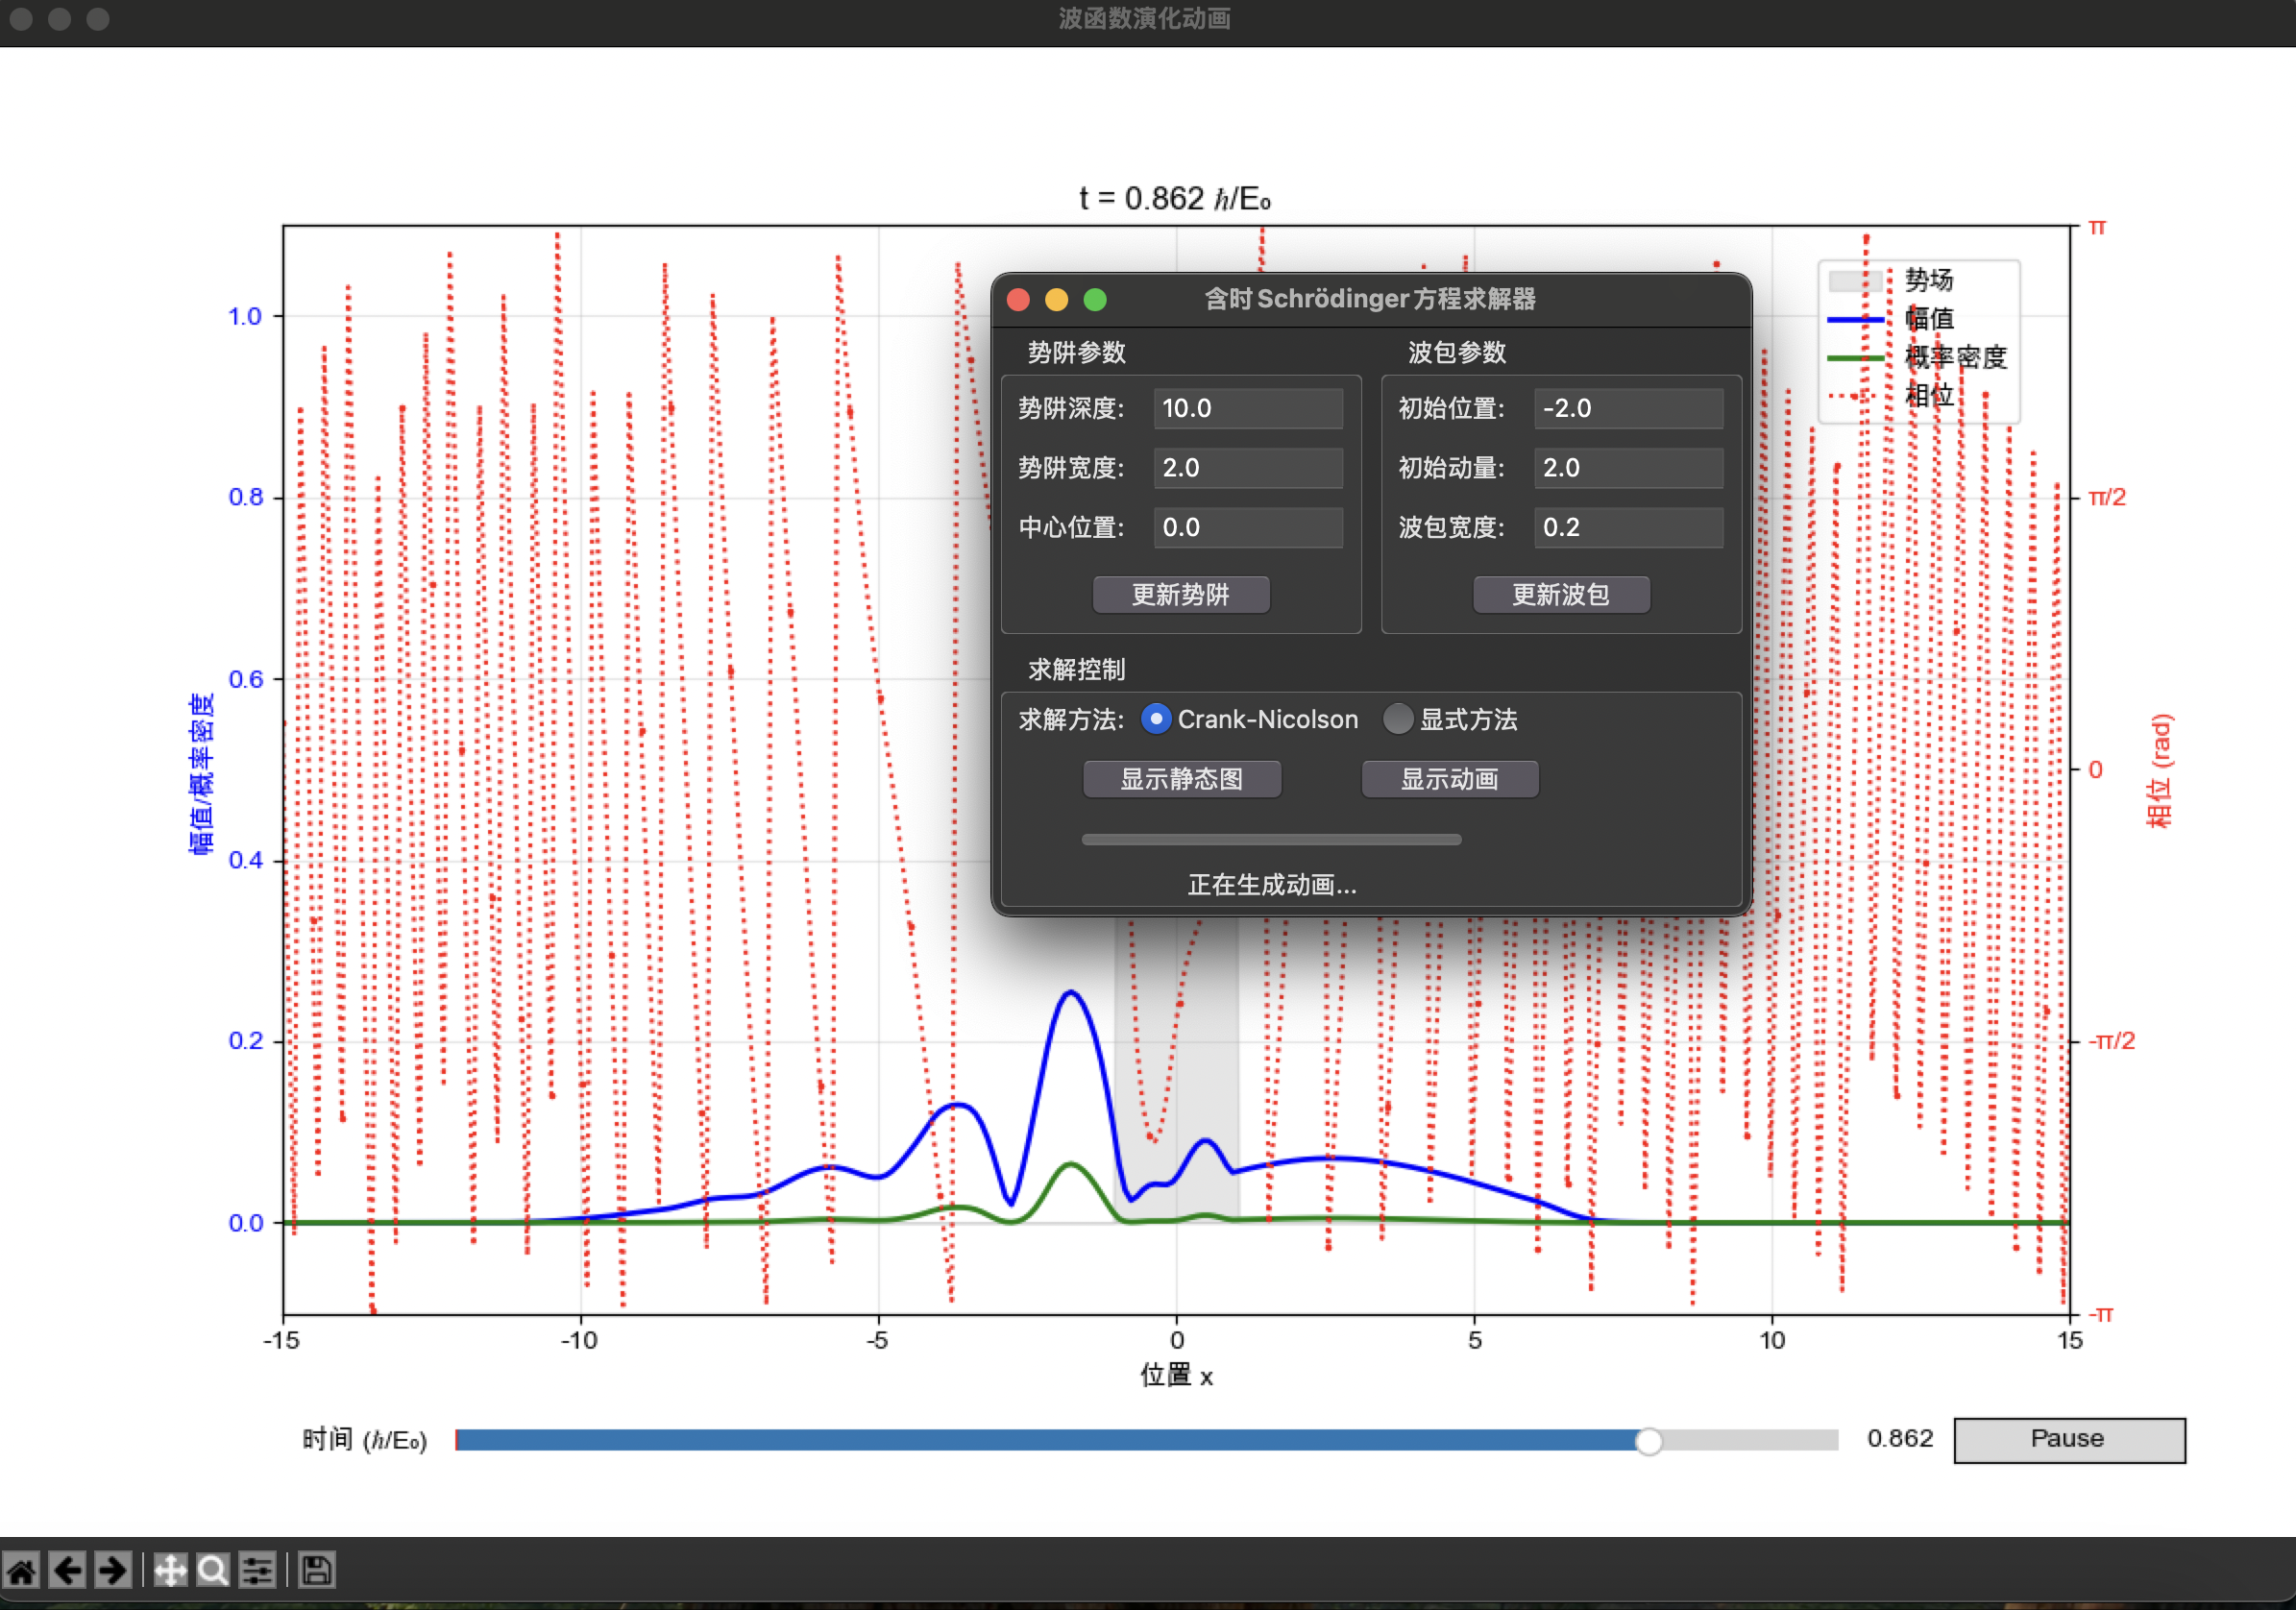
\includegraphics[width=1.0\textwidth]{Problem_2/figs/cn_anim.png}
    \caption{Crank–Nicolson解法中间态(动画截图)}
\end{figure}
本题使用的默认参数也可从图中读出,下图表明两种解法结果一致。动画运行需要先点击“显示动画”按钮,待动画生成就绪后会显示并自动播放,有进度条可供拖动回放。动画播放器存在一些已知bug,没力气修复了,不影响求解结果与静态图展示。
\begin{figure}[H]
    \centering
    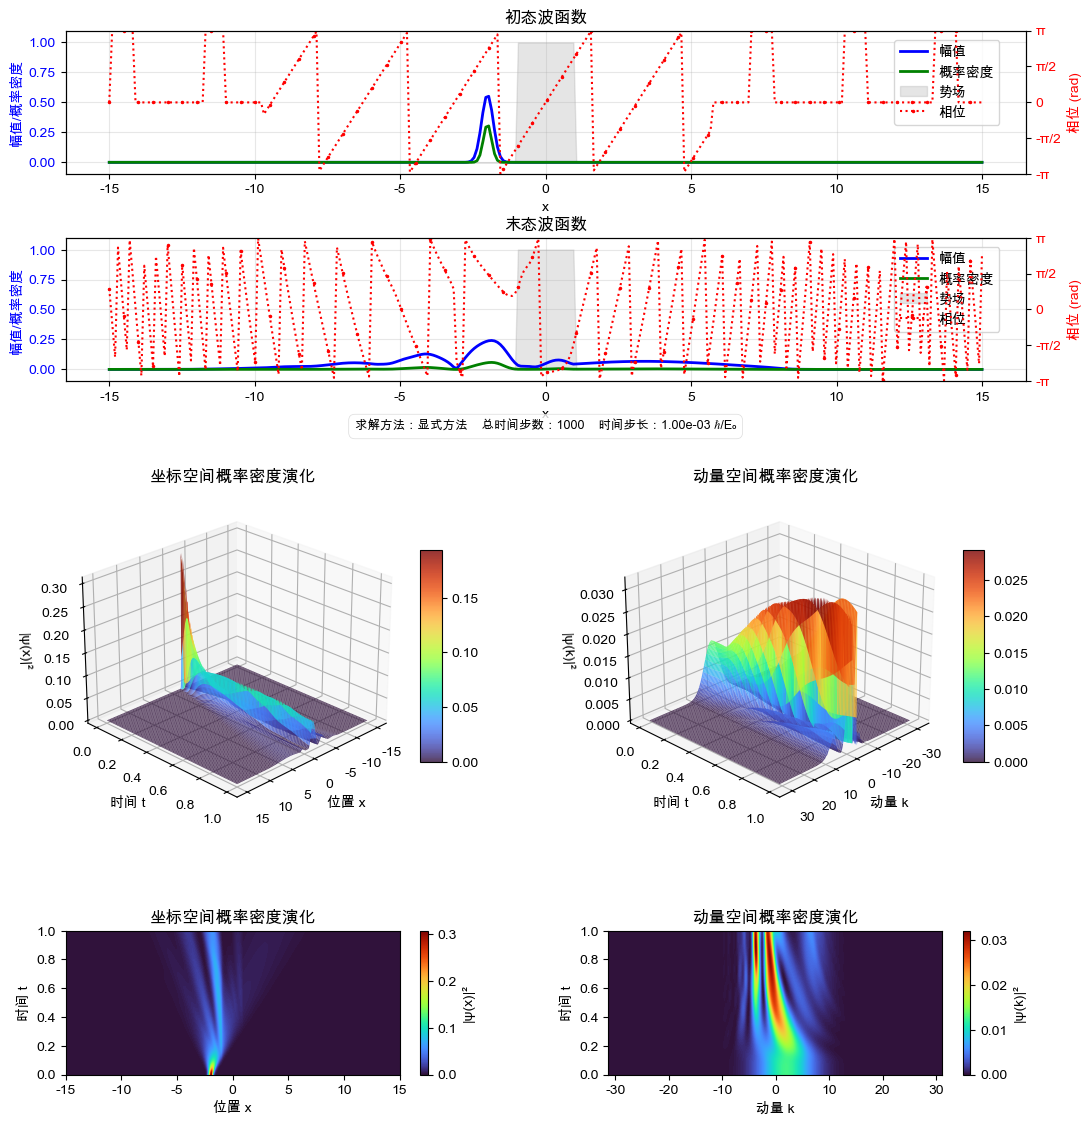
\includegraphics[width=1.0\textwidth]{Problem_2/figs/ex_result.png}
    \caption{显式解法结果}
\end{figure}